\documentclass[preprint,12pt]{elsarticle}
\usepackage{amsmath}
\usepackage{booktabs}
\usepackage{graphicx}
\usepackage{hyperref}
\usepackage{float}
\usepackage{xcolor}
\usepackage{makecell}
\usepackage{caption}
\usepackage{longtable}
\usepackage{booktabs}

\captionsetup[table]{font=normal}
\biboptions{authoryear}

\setlength{\parskip}{0.5em}
\renewcommand{\arraystretch}{1.2}

\journal{Economics Letters}

\begin{document}

\begin{frontmatter}

\title{Weakening Environmental Enforcement and Homicides: Evidence from Indigenous Territories in Brazil}

\author[u1]{Pedro Hemsley}
\author[u1]{Romero Rocha}
\author[u2]{Victor Libera}
\address[u1]{Universidade Federal do Rio de Janeiro, Brazil}
\address[u2]{Banco Nacional de Desenvolvimento Economico e Social (BNDES), Brazil}

\begin{abstract}
We study whether the post-2016 weakening of Brazil's federal environmental enforcement against illegal gold mining raised homicides where illegal-mining incentives concentrate. Using a 2010–2022 municipality-year panel restricted to Amazonia or Cerrado, we estimate a difference-in-differences-in-differences (DDD) model on the simultaneous overlap of Indigenous territory and gold reserve. Treated municipalities experience a post-2016 increase in homicide rates of about a third of a standard deviation, peaking in 2018. The result survives state-by-year fixed effects, alternative timing (2017), and population weighting; a dual-break specification rules out absorption of the 2013 deregulation shock of Pereira and Pucci (2026).
\end{abstract}

\begin{keyword}
Illegal mining \sep Indigenous territories \sep Violence \sep Difference-in-differences \sep Brazil
\end{keyword}

\end{frontmatter}

\section{Introduction}
Illegal gold mining is a major source of environmental and social harm in Brazil \citep{pereira_pucci_2024}. We focus on a specific cell where this problem concentrates: municipalities where Indigenous territories overlap known gold reserves, depicted in Figure~\ref{fig:map} as wine-colored. In those municipalities, high resource rents and contested land rights can intensify violent conflict; most lie in the Amazon and Cerrado biomes. Federal enforcement of mining bans is the binding constraint on illegal extraction, so shocks to the operational capacity of the enforcement agencies generate variation in the incentives to mine illegally.

\begin{figure}[H]
\centering
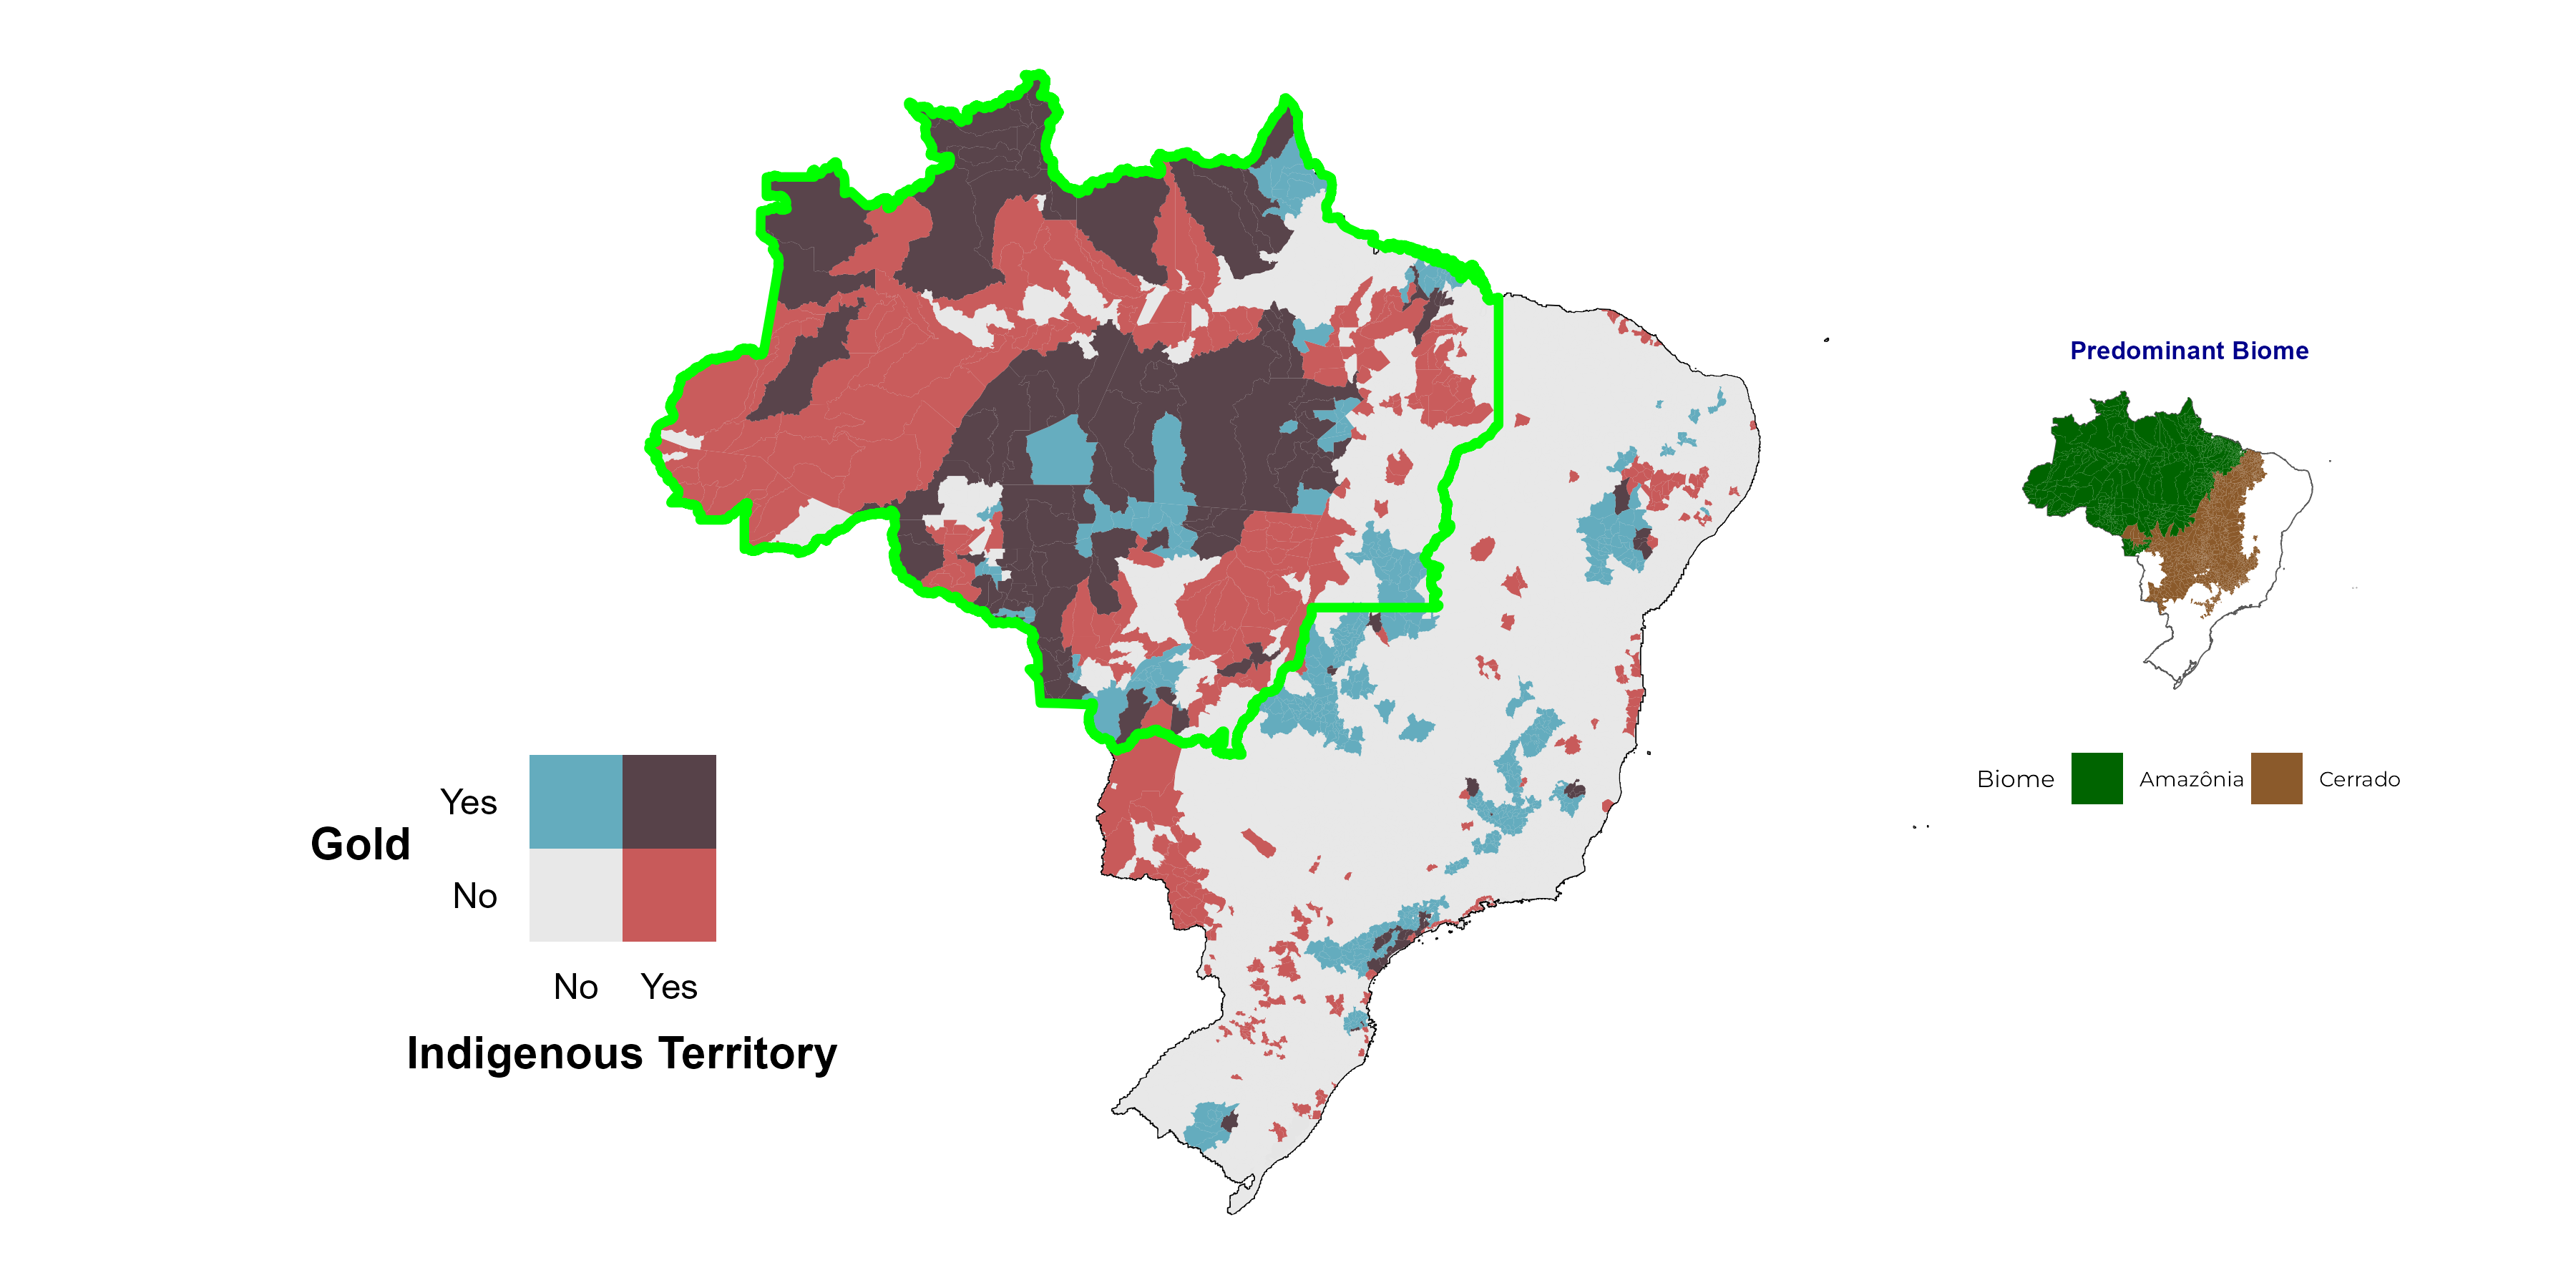
\includegraphics[width=0.88\textwidth]{figures/MapaTIOU.png}
\caption{Wine-colored municipalities are those overlapping both an Indigenous territory and a known gold reserve (Gold × IT $= 1$). The inset shows the Amazonia and Cerrado biomes.}
\label{fig:map}
\end{figure}

We study whether the post-2016 weakening of Brazilian federal environmental enforcement was associated with higher homicide rates in the municipalities where illegal-mining incentives are strongest. Using a 2010--2022 municipality-year panel restricted to municipalities overlapping Amazonia or Cerrado, we estimate a difference-in-differences-in-differences (DDD) model in which the treatment cell is the simultaneous overlap of an Indigenous territory ($IT=1$) and a known gold reserve ($Gold=1$) --- precisely the cell in which any gold extraction is necessarily illegal under Brazilian federal law (see Section~\ref{sec:background}). The triple interaction $Gold \times IT \times Post2016$ is 7.211 homicides per 100,000 inhabitants ($p=0.009$), or about 0.3 standard deviations of the cross-sectional homicide rate distribution, and peaks in 2018. The estimate is robust to alternative treatment timing (2017), to state-by-year fixed effects, to decomposition into simple DDs, and to population-weighted estimation.

Our note connects to two recent papers. \citet{nunes2024lessons} document a progressive weakening of the Brazilian command-and-control enforcement model during the late 2010s --- focused on crimes against the flora --- and identify 2018 as the institutional inflection point at which federal field inspections returned to the dispersed, pre-PPCDAm pattern. We show that the same period, and the same year, mark a sharp differential increase in homicides in the gold-rich Indigenous-territory cell, indicating that the institutional weakening they document for deforestation enforcement is also visible on the illegal-gold-mining margin. \citet{pereira_pucci_2024} study a 2013 deregulation that increased illegal gold mining and violence in Amazon municipalities exposed to gold deposits inside protected areas;\footnote{Our exercise differs from theirs in three respects: shock (post-2016 enforcement weakening vs.~the 2013 deregulation), design (DDD with $Gold \times TI$ as the treatment cell vs.~DiD with gold-deposits-inside-protected-areas as the treated group), and sample (Amazonia$+$Cerrado in 2010--2022 vs.~Amazon-only in 2006--2019).} we verify in dual-break specifications that our post-2016 effect is not relabeling their 2013 channel. More broadly, the paper connects to the literature on commodity rents, contested property rights, and local violence \citep{dube2013commodity,fetzer2017property,moreno2024technical,falcone2022modernization}. Our contribution is to show that the late-2010s weakening of environmental enforcement had a measurable violence cost on the illegal-gold-mining margin, separately from the 2013 market deregulation channel studied by Pereira and Pucci.

\section{Institutional background}\label{sec:background}

\subsection{Legal architecture}
Mining inside Indigenous territories is forbidden under Article 231, paragraph 3 of the 1988 Brazilian Federal Constitution, which conditions any such activity on specific authorization by the National Congress that has not been granted; small-scale gold mining (\textit{garimpo}) is further prohibited from operating within protected areas by Law 7.805/1989; and most categories of federal Conservation Units bar mining outright under the National System of Conservation Units (Law 9.985/2000). Gold deposits located inside an Indigenous territory therefore cannot be legally extracted, and the municipalities that simultaneously overlap an Indigenous territory and a known gold reserve are precisely those in which illegal-mining incentives concentrate.

\subsection{Federal enforcement agencies}
Federal enforcement of these mining bans is delivered by three agencies: IBAMA (the federal environmental enforcement agency), ICMBio (responsible for federal Conservation Units), and FUNAI (responsible for protecting Indigenous territories). Shocks to their operational capacity are therefore a natural source of variation in the incentives to mine illegally.

\subsection{The 2013 deregulation and the post-2016 enforcement weakening}

After the change in the federal political cycle in 2016 (Temer became interim president on May 12, 2016 and was confirmed on August 31, 2016) and the fiscal restriction adopted shortly thereafter, all three enforcement agencies saw substantial reductions in budget and personnel. IBAMA and ICMBio together lost on the order of one quarter of their staff over the period, with operational capacity for field inspections deteriorating in parallel; FUNAI also experienced sharp cuts to its budget and to its field-protection capacity in Indigenous territories \citep{abessa2019systematic,pereira2020brazilian,branford2017brazil}. \citet{nunes2024lessons} document that, against this institutional backdrop, the broader Brazilian command-and-control enforcement model weakened progressively during the late 2010s, identifying 2018 as the year in which federal field inspections returned to the dispersed, pre-PPCDAm pattern, with sharp drops in infraction notices, embargoes and asset confiscations thereafter.

 \citet{pereira_pucci_2024} document a previous, 2013 deregulation that exempted gold first-buyers (PCOs, the regulated stores that act as the legal entry point of raw gold into the financial system) from liability for the origin of the gold they purchased, and show that the deregulation raised illegal gold mining and violence in Amazon municipalities exposed to gold deposits located inside protected areas.

\section{Data and empirical strategy}\label{sec:strategy}
\subsection{Data}
We use a municipality-year panel from 2010 to 2022. The outcome is homicide rate per 100,000 inhabitants, constructed from SIM/DATASUS mortality records and estimated municipal population data. We combine those data with geospatial indicators:
\begin{itemize}
\item \(IT_i=1\): municipality overlaps at least one official Indigenous territory polygon.
\item \(Gold_i=1\): municipality overlaps at least one known gold-reserve polygon.
\end{itemize}

A more detailed discussion of how each variable was constructed is provided in the online supplementary material. The sample is restricted to municipalities that overlap Amazonia or Cerrado (any-overlap definition from IBGE municipality-biome correspondence) and contains 24,358 municipality-year observations (1,874 municipalities over 13 years).

\subsection{Baseline DDD}
Our baseline specification is
\begin{equation}
\begin{aligned}
y_{it} =\;& \beta_1(Gold_i \times Post_t) + \beta_2(IT_i \times Post_t) + \beta_3(Gold_i \times IT_i \times Post_t) \\
&+ \mu_i + \lambda_t + \varepsilon_{it}
\end{aligned}
\end{equation}
where \(y_{it}\) is homicide rate, \(\mu_i\) are municipality fixed effects, and \(\lambda_t\) are year fixed effects. We use $Post_t = \mathbf{1}\{t \geq 2016\}$ as our baseline treatment indicator, anchored on the change in the federal political cycle, and report estimates with $Post_t = \mathbf{1}\{t \geq 2017\}$ as a robustness check. We focus on municipalities in Amazonia or Cerrado, the biomes most directly connected to environmental conflict.\footnote{Main results hold if the exercise is restricted to the Legal Amazon, and they also hold if all Brazilian municipalities are included. In particular, using all municipalities yields very similar DDD estimates: 8.685 (s.e. 2.715) with treatment starting in 2016 and 8.885 (s.e. 2.814) with treatment starting in 2017. We prefer the Amazonia $+$ Cerrado sample because it targets the environmentally relevant municipalities and yields cleaner dynamic patterns.} Standard errors are clustered by municipality. The coefficient of interest is \(\beta_3\).

\subsection{Dual-break DDD}
To separate the post-2016 effect from the 2013 channel emphasized by \citet{pereira_pucci_2024}, we estimate a piecewise specification that allows the DDD interaction to shift at two distinct breaks, 2013 and 2016 (or, alternatively, 2017):
\begin{equation}
\begin{aligned}
y_{it} = & \sum_{b \ \in \ \{2013, \ 2016\}} \\
&\left[ \beta_{1b}(Gold_i \times Post^b_t) + \beta_{2b}(IT_i \times Post^b_t) \right. \left. + \beta_{3b}(Gold_i \times IT_i \times Post^b_t) \right] \\
&+ \mu_i + \lambda_t + \varepsilon_{it}.
\end{aligned}
\end{equation}

In this specification, \(Post^{2013}_t\) and \(Post^{2016}_t\) are nested step indicators, so \(\beta_{3,2013}\) captures the differential change in homicide rates of treated municipalities that turns on in 2013 and persists thereafter, while \(\beta_{3,2016}\) captures the additional incremental change from 2016 onward, on top of any 2013 effect. The total post-2016 DDD effect is therefore \(\beta_{3,2013}+\beta_{3,2016}\). If our 2016 estimate is just relabeling the 2013 channel, $\beta_{3,2016}$ should shrink toward zero once $\beta_{3,2013}$ is allowed to enter. We report analogous estimates replacing 2016 with 2017.

\section{Results}
\subsection{Main estimates}
Table~\ref{tab:main} reports core estimates. In the main model (post-2016), the triple interaction is 7.211 (s.e. 2.757, \(p=0.009\)), corresponding to approximately 0.3 standard deviations of the cross-sectional homicide rate distribution in the sample. With treatment starting in 2017, it is 7.767 (s.e. 2.947, \(p=0.008\)).

We also estimate non-linear state trends via state-by-year fixed effects. The post-2016 triple interaction remains positive and statistically significant: 8.691 (s.e. 2.727, \(p=0.001\)).

\begin{table}[H]
\caption{Main DDD Estimates in Amazônia $+$ Cerrado Municipalities (2010$-$2022)}
\label{tab:main}
\centering
\setlength{\tabcolsep}{3.5pt}
\renewcommand{\arraystretch}{1.2}
\resizebox{\textwidth}{!}{%\begin{tabular}{lccc}
%\toprule
%& \multicolumn{3}{c}{Dependent variable: Homicide rate per 100,000} \\
%\cmidrule(lr){2-4}
%& Post>=2016 & Post>=2017 & Post>=2016 + state-year FE \\
%& (1) & (2) & (3) \\
%\midrule
%Gold $\times$ Post & 2.529* & 2.886** & 1.750 \\
% & (1.332) & (1.388) & (1.354) \\
%TI $\times$ Post & -0.152 & 0.414 & -2.381* \\
% & (1.133) & (1.118) & (1.394) \\
%Gold $\times$ TI $\times$ Post & 8.769** & 8.806** & 9.711*** \\
% & (3.419) & (3.550) & (3.470) \\
%\midrule
%Municipality FE & Yes & Yes & Yes \\
%Year FE & Yes & Yes & No \\
%State-year FE & No & No & Yes \\
%Observations & 17524 & 17524 & 17511 \\
%Within R\textsuperscript{2} & 0.007 & 0.008 & 0.005 \\
%\midrule
%\multicolumn{4}{l}{\footnotesize Clustered standard errors by municipality in parentheses.} \\
%\multicolumn{4}{l}{\footnotesize *** p<0.01, ** p<0.05, * p<0.1.} \\
%\bottomrule
%\end{tabular}

{\fontsize{7}{8}\selectfont
\begin{tabular}{lccc}
\toprule
& \multicolumn{3}{c}{Dependent Variable: Homicide Rate per 100,000} \\
\cmidrule(lr){2-4}
& Post $\geq$ 2016 & Post $\geq$ 2017 & \makecell{Post $\geq$ 2016 $+$ \\ State-year FE} \\
& (1) & (2) & (3) \\
\midrule
Gold $\times$ Post & 2.662** & 2.761** & 0.884 \\ 
& (1.065) & (1.138) & (1.125) \\
IT $\times$ Post & -0.343 & 0.214 & -2.673** \\
& (1.005) & (0.989) & (1.202) \\
Gold $\times$ IT $\times$ Post & 7.211*** & 7.767*** & 8.691*** \\
 & (2.757) & (2.947) & (2.727) \\
\midrule
Municipality FE & Yes & Yes & Yes \\
Year FE & Yes & Yes & No \\
State-year FE & No & No & Yes \\
Observations & 24,358 & 24,358 & 24,358 \\
\midrule
\multicolumn{4}{l}{ Standard errors in parentheses.} \\
\multicolumn{4}{l}{ *** p $<$ 0.01, ** p $<$ 0.05, * p $<$ 0.1.} \\
\bottomrule
\end{tabular}
}}
\end{table}

To improve interpretation, we decompose the DDD into simple DDs. Within \(IT=1\) municipalities, the DD effect of \(Gold\times Post2016\) is 9.874 (\(p<0.001\)), while within \(IT=0\) it is 2.662 (\(p=0.012\)). Symmetrically, within \(Gold=1\), the DD effect of \(IT\times Post2016\) is 6.867 (\(p=0.008\)), versus -0.343 (\(p=0.732\)) within \(Gold=0\). This pattern is consistent with the DDD estimate.

Additional robustness checks are also supportive. Population-weighted DDD estimates are 9.504 (\(p=0.014\)) with municipality and year FE, and 7.221 (\(p=0.042\)) with municipality and state-by-year FE. Tests for differential pre-trends within the pre-period --- using only data through 2015 with hypothetical intervention dates in 2013 and 2014 --- are not statistically significant (\(p=0.113\) and \(p=0.411\)).

Table~\ref{tab:dual} reports dual-break estimates. Once both breaks are included, the 2013 effect is always small and imprecise. By contrast, the incremental post-2016 effect ranges from 5.617 to 6.905 and remains statistically significant; with a 2017 second break, the incremental effect ranges from 6.348 to 7.379. The later enforcement-weakening component is therefore not mechanically absorbing the earlier 2013 deregulation channel.

\begin{table}[H]
\caption{Dual-break DDD Estimates}
\label{tab:dual}
\centering
\footnotesize
\setlength{\tabcolsep}{4pt}
\renewcommand{\arraystretch}{1.2}
\resizebox{\textwidth}{!}{{\fontsize{10}{12}\selectfont
\begin{tabular}{lccc}
\toprule
Specification & 2013 Effect & \makecell{Increment After \\ Second Break} & Total Later Effect \\
\midrule
2013 $+$ 2016 breaks & 3.187 & 5.617** & 8.804*** \\
 & (2.219) & (2.765) & (3.167) \\
2013 $+$ 2016 breaks $+$ State-year FE & 3.571 & 6.905** & 10.477*** \\
 & (2.266) & (2.834) & (3.067) \\
2013 + 2017 breaks & 3.310 & 6.348** & 9.659** \\
 & (2.204) & (2.924) & (3.416) \\
2013 $+$ 2017 breaks $+$ State-year FE & 3.977* & 7.379** & 11.356*** \\
 & (2.246) & (3.062) & (3.335) \\
\midrule
\multicolumn{4}{l}{ The first column is the DDD effect after 2013 and before the second break.} \\
\multicolumn{4}{l}{ Clustered standard errors by municipality in parentheses.} \\
\multicolumn{4}{l}{ *** p $<$ 0.01, ** p $<$ 0.05, * p $<$ 0.1.} \\
\bottomrule
\end{tabular}
}}
\end{table}

\subsection{Dynamic evidence and pre-trends}
Figure~\ref{fig:event} shows dynamic DDD coefficients for the triple interaction, with 2015 as reference year. Coefficients for 2010--2014 are jointly insignificant in both baseline and state-year FE specifications (\(p=0.451\) and \(p=0.672\)). Post-treatment effects are strongest in 2018 (10.984, \(p=0.005\)) and remain positive in subsequent years, though less precisely estimated. The fact that the largest differential effect on homicide rates occurs in 2018 lines up directly with the institutional inflection identified by \citet{nunes2024lessons}.

\begin{figure}[H]
\centering

\includegraphics[width=0.88\textwidth]{7. Mining Deregulation and Homicides/figures/DynamicDDD.png}
\caption{Dynamic DDD event-study (reference year: 2015)}
\label{fig:event}
\end{figure}

\section{Conclusion}
In municipalities located in Amazonia or Cerrado, homicide rates rose after the 2016 political-cycle change specifically where Indigenous-territory overlap and gold-reserve overlap coexist, with the differential increase peaking in 2018 --- the year that \citet{nunes2024lessons} identify as the inflection point of Brazil's federal environmental-enforcement model. The result is robust to treatment-year coding (2016 vs. 2017), to non-linear state trends, to decomposition into simple DDs, to within-pre-period falsification tests, and to population-weighted estimation.

Dual-break results indicate that this pattern is not mechanically capturing the 2013 deregulation effect documented by \citet{pereira_pucci_2024}: once both breaks are included, the incremental post-2016/post-2017 effect remains large and significant, whereas the 2013-only component is small and imprecise.

This evidence is consistent with the view that weaker effective enforcement in environmentally sensitive and resource-rich territories can generate substantial local violence costs.

\section*{Data availability}
All data used in the paper are drawn from publicly available sources: mortality records (SIM/DATASUS), municipal population estimates and biome correspondence (Brazilian Institute of Geography and Statistics, IBGE), Indigenous territory polygons (National Foundation of Indigenous Peoples, FUNAI), and gold provinces and districts (Geological Survey of Brazil, SGB). The assembled municipality-year panel and replication code will be deposited in a public repository (OSF/Zenodo) upon request.

\section*{Declaration of generative AI and AI-assisted technologies in the writing process}

During the preparation of this work, the authors used Claude (Anthropic) for the following tasks: (i) reviewing the manuscript text and suggesting edits; (ii) searching online references and databases relevant to the institutional background; (iii) reviewing the manuscript against the journal's requirements and the relevant literature; and (iv) reviewing the replication code and suggesting adjustments. After using this tool, the authors reviewed and edited the content as needed and take full responsibility for the content of the publication.

\bibliographystyle{elsarticle-harv}
\bibliography{references}

\appendix

\section{Data} \label{ap:data}

This paper is based on three constructed variables: homicide rate per 100,000 inhabitants, a binary variable for gold mining reserves in the municipality, and a binary variable for indigenous territories in the municipality. Therefore, it is worth highlighting their composition and possible limitations.     

\subsection*{A.1. Homicide Rate}

The homicide rate is the simple ratio of homicides to population, multiplied by 100,000.

\begin{itemize}
    \item In the numerator, homicide is defined as the sum of three ICD-10 cause-of-death categories, by municipality of occurrence: assaults (X85–Y09), events of undetermined intent (Y10–Y34), and legal interventions (Y35). The raw data was sourced from SIM/DATASUS.
    
    \item In the denominator, population figures are estimated by the Brazilian Institute of Geography and Statistics (IBGE) for the Federal Court of Accounts (TCU), within the scope of the Municipalities Participation Fund (FPM), by municipality of residence. The data is available on the IBGE website.
\end{itemize}

It is worth mentioning some points. First, the numerator is measured by the municipality of \textit{occurrence} while the denominator is measured by the municipality of \textit{residence}. Although SIM/DATASUS allows, by default, the retrieval of deaths by municipality of residence, we opted for a perspective based on occurrence. The underlying reasoning is that municipalities where Indigenous territories overlap gold reserves often have a substantial share of inhabitants whose residence is outside the municipality –- that is, low-skilled workers who migrate from their places of residence in search of increased income from high rents of natural resources. In contrast, only IBGE's population estimates are available at the municipal level, and they only consider the perspective of residence.

Second, other ICD-10 cause-of-death categories could be used to build the homicide variable -- or even some category could be removed. The existing literature often addresses homicides as a combination of one or more of the mentioned categories, in addition to intentional self-harm (X60-X84). We opted to include the three most used ICD-10 cause-of-death categories. A comprehensive table with all ICD-10 definitions ranging from X60 to Y35 is displayed for consultation.

\begingroup
\small
\renewcommand{\arraystretch}{1.2}
\setlength{\tabcolsep}{3.5pt}
% icd10_table.tex
% ICD-10 Codes X60-Y35 grouped by official WHO blocks
% Required packages in main document:
%   \usepackage{longtable}
%   \usepackage{booktabs}

\begin{longtable}{p{2.2cm} p{10.3cm}}

\caption{International Statistical Classification of Diseases and Related Health Problems - 10th Revision (ICD-10): Codes X60--Y35}
\label{tab:icd10_x60_y35} \\

\toprule
\textbf{Code} & \textbf{Description} \\
\midrule
\endfirsthead

\multicolumn{2}{l}{\small\itshape (Continued from previous page)} \\[2pt]
\toprule
\textbf{Code} & \textbf{Description} \\
\midrule
\endhead

\midrule
\multicolumn{2}{r}{\small\itshape (Continued on next page)} \\
\endfoot

\bottomrule
\endlastfoot

% ================================================================
% BLOCK X60-X84  Intentional self-harm
% ================================================================
\multicolumn{2}{l}{\textbf{X60--X84 \quad Intentional Self-Harm}} \\
\midrule
\texttt{X60} & Intentional self-poisoning by and exposure to nonopioid analgesics, antipyretics and antirheumatics \\
\texttt{X61} & Intentional self-poisoning by and exposure to antiepileptic, sedative-hypnotic, antiparkinsonism and psychotropic drugs, not elsewhere classified \\
\texttt{X62} & Intentional self-poisoning by and exposure to narcotics and psychodysleptics (hallucinogens), not elsewhere classified \\
\texttt{X63} & Intentional self-poisoning by and exposure to other drugs acting on the autonomic nervous system \\
\texttt{X64} & Intentional self-poisoning by and exposure to other and unspecified drugs, medicaments and biological substances \\
\texttt{X65} & Intentional self-poisoning by and exposure to alcohol \\
\texttt{X66} & Intentional self-poisoning by and exposure to organic solvents and halogenated hydrocarbons and their vapours \\
\texttt{X67} & Intentional self-poisoning by and exposure to other gases and vapours \\
\texttt{X68} & Intentional self-poisoning by and exposure to pesticides \\
\texttt{X69} & Intentional self-poisoning by and exposure to other and unspecified chemicals and noxious substances \\
\texttt{X70} & Intentional self-harm by hanging, strangulation and suffocation \\
\texttt{X71} & Intentional self-harm by drowning and submersion \\
\texttt{X72} & Intentional self-harm by handgun discharge \\
\texttt{X73} & Intentional self-harm by rifle, shotgun and larger firearm discharge \\
\texttt{X74} & Intentional self-harm by other and unspecified firearm and gun discharge \\
\texttt{X75} & Intentional self-harm by explosive material \\
\texttt{X76} & Intentional self-harm by smoke, fire and flames \\
\texttt{X77} & Intentional self-harm by steam, hot vapours and hot objects \\
\texttt{X78} & Intentional self-harm by sharp object \\
\texttt{X79} & Intentional self-harm by blunt object \\
\texttt{X80} & Intentional self-harm by jumping from a high place \\
\texttt{X81} & Intentional self-harm by jumping or lying before moving object \\
\texttt{X82} & Intentional self-harm by crashing of motor vehicle \\
\texttt{X83} & Intentional self-harm by other specified means \\
\texttt{X84} & Intentional self-harm by unspecified means \\[6pt]

% ================================================================
% BLOCK X85-Y09  Assault
% ================================================================
\multicolumn{2}{l}{\textbf{X85--Y09 \quad Assault}} \\
\midrule
\texttt{X85} & Assault by drugs, medicaments and biological substances \\
\texttt{X86} & Assault by corrosive substance \\
\texttt{X87} & Assault by pesticides \\
\texttt{X88} & Assault by gases and vapours \\
\texttt{X89} & Assault by other specified chemicals and noxious substances \\
\texttt{X90} & Assault by unspecified chemical or noxious substance \\
\texttt{X91} & Assault by hanging, strangulation and suffocation \\
\texttt{X92} & Assault by drowning and submersion \\
\texttt{X93} & Assault by handgun discharge \\
\texttt{X94} & Assault by rifle, shotgun and larger firearm discharge \\
\texttt{X95} & Assault by other and unspecified firearm and gun discharge \\
\texttt{X96} & Assault by explosive material \\
\texttt{X97} & Assault by smoke, fire and flames \\
\texttt{X98} & Assault by steam, hot vapours and hot objects \\
\texttt{X99} & Assault by sharp object \\
\texttt{Y00} & Assault by blunt object \\
\texttt{Y01} & Assault by pushing from high place \\
\texttt{Y02} & Assault by pushing or placing victim before moving object \\
\texttt{Y03} & Assault by crashing of motor vehicle \\
\texttt{Y04} & Assault by bodily force \\
\texttt{Y05} & Sexual assault by bodily force \\
\texttt{Y06} & Neglect and abandonment \\
\texttt{Y07} & Other maltreatment syndromes \\
\texttt{Y08} & Assault by other specified means \\
\texttt{Y09} & Assault by unspecified means \\[6pt]

% ================================================================
% BLOCK Y10-Y34  Event of undetermined intent
% ================================================================
\multicolumn{2}{l}{\textbf{Y10--Y34 \quad Event of Undetermined Intent}} \\
\midrule
\texttt{Y10} & Poisoning by and exposure to nonopioid analgesics, antipyretics and antirheumatics, undetermined intent \\
\texttt{Y11} & Poisoning by and exposure to antiepileptic, sedative-hypnotic, antiparkinsonism and psychotropic drugs, not elsewhere classified, undetermined intent \\
\texttt{Y12} & Poisoning by and exposure to narcotics and psychodysleptics (hallucinogens), not elsewhere classified, undetermined intent \\
\texttt{Y13} & Poisoning by and exposure to other drugs acting on the autonomic nervous system, undetermined intent \\
\texttt{Y14} & Poisoning by and exposure to other and unspecified drugs, medicaments and biological substances, undetermined intent \\
\texttt{Y15} & Poisoning by and exposure to alcohol, undetermined intent \\
\texttt{Y16} & Poisoning by and exposure to organic solvents and halogenated hydrocarbons and their vapours, undetermined intent \\
\texttt{Y17} & Poisoning by and exposure to other gases and vapours, undetermined intent \\
\texttt{Y18} & Poisoning by and exposure to pesticides, undetermined intent \\
\texttt{Y19} & Poisoning by and exposure to other and unspecified chemicals and noxious substances, undetermined intent \\
\texttt{Y20} & Hanging, strangulation and suffocation, undetermined intent \\
\texttt{Y21} & Drowning and submersion, undetermined intent \\
\texttt{Y22} & Handgun discharge, undetermined intent \\
\texttt{Y23} & Rifle, shotgun and larger firearm discharge, undetermined intent \\
\texttt{Y24} & Other and unspecified firearm discharge, undetermined intent \\
\texttt{Y25} & Contact with explosive material, undetermined intent \\
\texttt{Y26} & Exposure to smoke, fire and flames, undetermined intent \\
\texttt{Y27} & Contact with steam, hot vapours and hot objects, undetermined intent \\
\texttt{Y28} & Contact with sharp object, undetermined intent \\
\texttt{Y29} & Contact with blunt object, undetermined intent \\
\texttt{Y30} & Falling, jumping or pushed from a high place, undetermined intent \\
\texttt{Y31} & Falling, lying or running before or into moving object, undetermined intent \\
\texttt{Y32} & Crashing of motor vehicle, undetermined intent \\
\texttt{Y33} & Other specified events, undetermined intent \\
\texttt{Y34} & Unspecified event, undetermined intent \\[6pt]

% ================================================================
% BLOCK Y35  Legal intervention (partial)
% ================================================================
\multicolumn{2}{l}{\textbf{Y35--Y36 \quad Legal Intervention and Operations of War (partial)}} \\
\midrule
\texttt{Y35} & Legal intervention \\*

\end{longtable}
\endgroup

\subsection*{A.2. Gold Reserves}

Based on \citet{sgb2024}, gold-bearing metallogenic provinces can be defined as regions where mineral occurrences and deposits appear in greater quantities or tonnage than neighboring areas, delimited by geologic-stratigraphic-tectonic boundaries, while districts are subdivisions of provinces, grouping spatially and genetically related deposits and occurrences. Therefore, we define \(Gold = 1\) for any municipality that overlaps at least one province or district of gold, considering that a district is not necessarily within a province. The polygons were obtained from the website of the Geological Survey of Brazil (SGB) in 2024.

\subsection*{A.3. Indigenous Territories}

The binary variable for indigenous territories was constructed based on the dataset of polygons of Indigenous territories made publicly available by National Foundation of Indigenous People (FUNAI) at GeoServer website. Therefore, we define \(IT = 1\) for any municipality that overlaps at least one indigenous territory in 2024.

\end{document}

